% Chapter 1

\chapter{Literature Review} % Write in your own chapter title
\label{Chapter1}
\lhead{Chapter 1. \emph{Literature Review}} % Write in your own chapter title to set the page header

\section{Introduction}
A power inverter, or inverter, is an electronic device that converts direct current (DC) to alternating current (AC).
The input voltage, output voltage and frequency, and overall power handling depend on the design of the specific circuitry[1].\\ 
Inverters can be divided into two kinds:
\begin{itemize}
\item Voltage Source Inverters (VSI)
\item Current Source Inverters (CSI)
\end{itemize}
\begin{figure}[htbp]
	\centering
		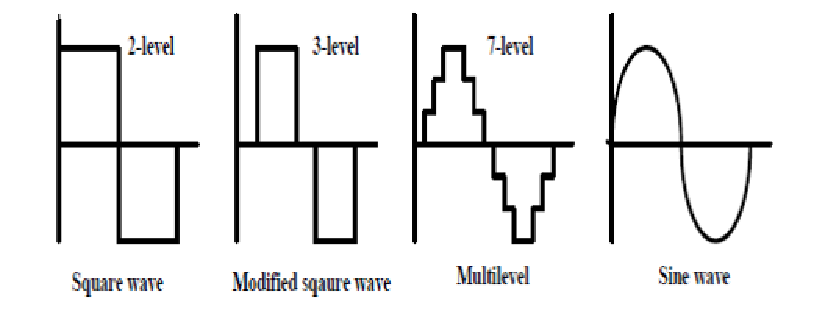
\includegraphics[width = 4in]{./Figures/Picture1.pdf}
		\rule{35em}{5pt}
	\caption{Outputs of Inverters}
	\label{fig:1}
\end{figure}
The basic component of an inverter is fast working switch like IGBT or MOSFET.However, later is more preferred because main advantage of a MOSFET is that it requires almost no input current to control the load current, when compared with IGBT.
\subsection{MOSFET}
The MOSFET\ref{fig:2} is a type of field-effect transistor (FET), most commonly fabricated by the controlled oxidation of silicon. It has an insulated gate, whose voltage determines the conductivity of the device. This ability to change conductivity with the amount of applied voltage can be used for amplifying or switching electronic signals.\\
The Mosfet is further divided into n-channel Mosfet and p-channel Mosfet depending upon formation and has three modes of opertion as :
\begin{itemize}
\item Cutoff mode
\item Ohmic mode
\item Active mode
\end{itemize}
For switciing purposes Mosfet is used in active and cutoff mode.
  \begin{figure}[htbp]
	\centering
		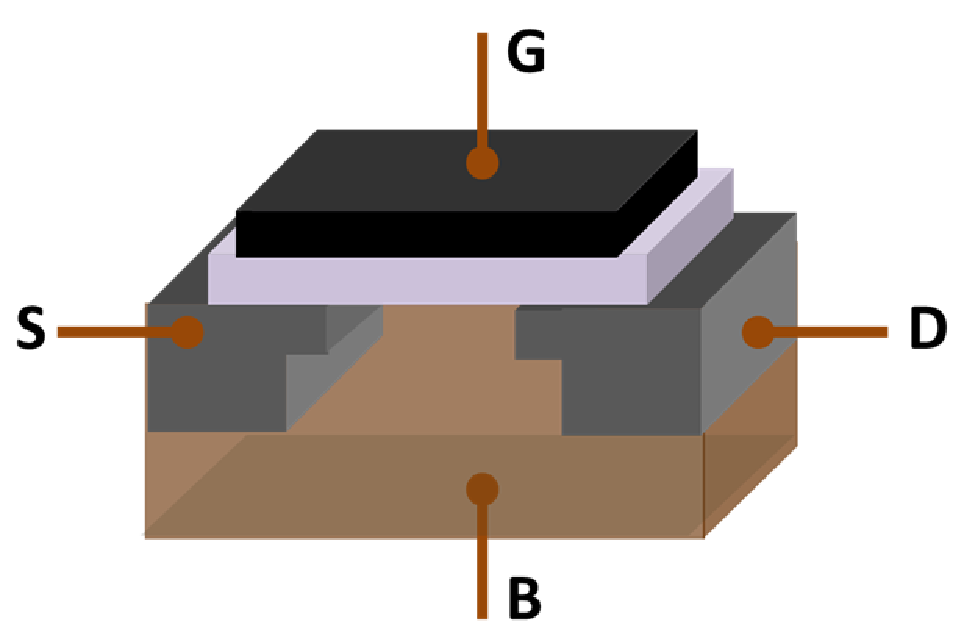
\includegraphics[width = 2in]{./Figures/Mosfet.pdf}
		\rule{35em}{5pt}
	\caption{ MOSFET showing gate (G), body (B), source (S) and drain (D) terminals. The gate is separated from the body by an insulating layer (white)}
	\label{fig:2}
\end{figure}
\section{Hierarchy of Inverter}
General Hierarchy of inverter\ref{fig:3} is shown below.Under the perspective of project the selective hierarchy will start from basic inverter to unequal dc sources cascaded h-bridge multilevel inverters.   
\begin{figure}[htbp]
	\centering
		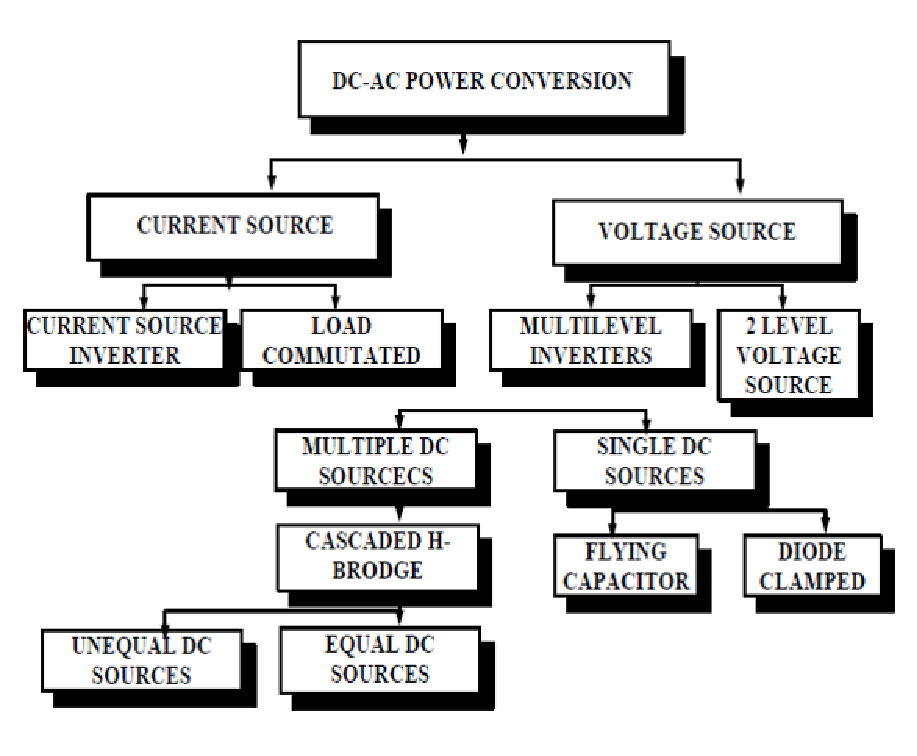
\includegraphics[width = 3in]{./Figures/Picture2.pdf}
		\rule{35em}{5pt}
	\caption{Hierarchy of inverter}
	\label{fig:3}
\end{figure}
\section{Voltage Source Inverter}
 If the input dc is voltage source, the inverter is called a voltage
source inverter.The VSI circuit has direct control over output (ac)
voltage. Shape of voltage wave-forms output by an ideal VSI should be independent of load connected at the output.\\
The simplest dc voltage source for a VSI may be a battery bank, which may consist of several cells in series-parallel combination.A voltage source is called stiff, if the source voltage magnitude does not depend on load connected to it. All VSI assume stiff voltage supply at the input.Some examples where voltage source inverters are used are: UPS units, adjustable speed drives (Automatic Star Delta) for ac motors, electronic frequency changer circuits etc.\\
The achievable magnitude of ac voltage is limited by the magnitude of inputc dc voltage. In some cases the inverter output voltage is stepped up using a transformer to meet the load requirement. 
VSI is further divided into two types:
\begin{itemize}
\item Multilevel Inverters
\item 2 Level Voltage Source
\end{itemize}
\section{Multilevel Inverters}
A multilevel inverter is a PE device which is capable of providing desired alternating voltage level at the output using multiple lower level DC voltages as an input.Multilevel inverters also enables the use of low power application in renewable energy sources.
These converters are suitable in high voltage and high power
applications due to:
\begin{itemize}
\item Their ability to synthesize higher voltages with a
limited maximum device rating
\item Less harmonic distortion
\item Producing of smaller common-mode voltage
\item Less electromagnetic compatibility problems
\item Attain higher voltage with a limited maximum device rating.
\end{itemize}
The range of the output power is a very important and evident
limitation of two-level inverter. However, this problem can be
overcome by introducing the concept of multilevel inverters.\\
The three most popular multilevel inverters are:
\begin{itemize}
\item Diode-Clamped Multilevel Inverter (DC-MLI)
\item Flying-Capacitor Multilevel Inverter (FC-MLI)
\item Cascaded H-Bridge Multilevel Inverter (CHBMLI)
\end{itemize}
First two use single voltage source for working while CHBMLI use multiple voltage sources.
\begin{figure}[htbp]
	\centering
		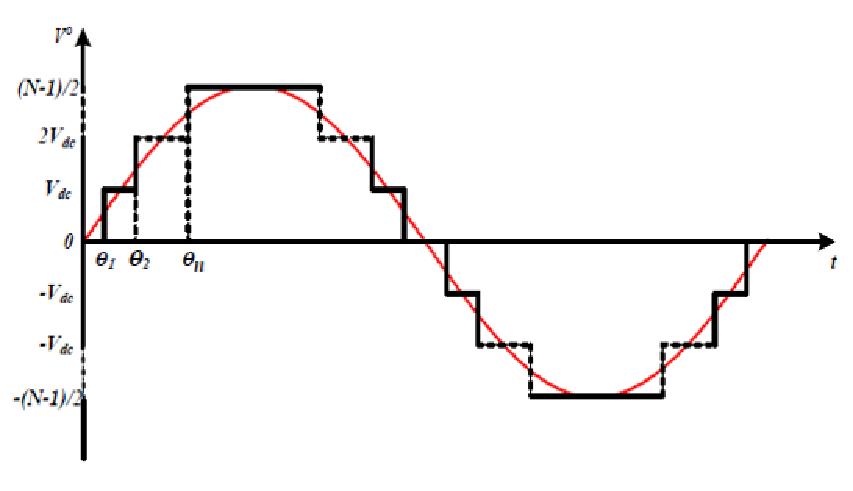
\includegraphics[width = 5in]{./Figures/Picture3.pdf}
		\rule{35em}{5pt}
	\caption{Generalized stepped waveform of multilevel inverters }
	\label{fig:4}
\end{figure}
 
\section{H Bridge}An H bridge \ref{fig:4} enables a reverse voltage to be applied across a load.\\
These circuits are often used in multiple applications to allow bidirectional movement of DC motors,
DC-to-AC converters,AC/AC converters,DC-to-DC $push–pull$ converter and many other kinds of power electronics use H bridges.\\
 An H bridge is built with four switches \ref{fig:2}. When the switches S1 and S4 are closed (and S2 and S3 are open) a positive voltage will be applied across the motor and vice versa. The point to ponder is that switches S1 and S2 should never be closed at the same time, as this would cause a short circuit on the input voltage source as seen from the figure. The same applies to the switches S3 and S4.\\
 Thus, functioning of a single H-bridge is similar to that of
conventional 2-level inverter. Each H-bridge requires an
isolated dc source/capacitor to generate its corresponding
output. The switches are activated in such a way that the
output voltage across the load terminals is the aggregation
of the voltage generated by the H-bridge.
 
\begin{figure}[htbp]
	\centering
		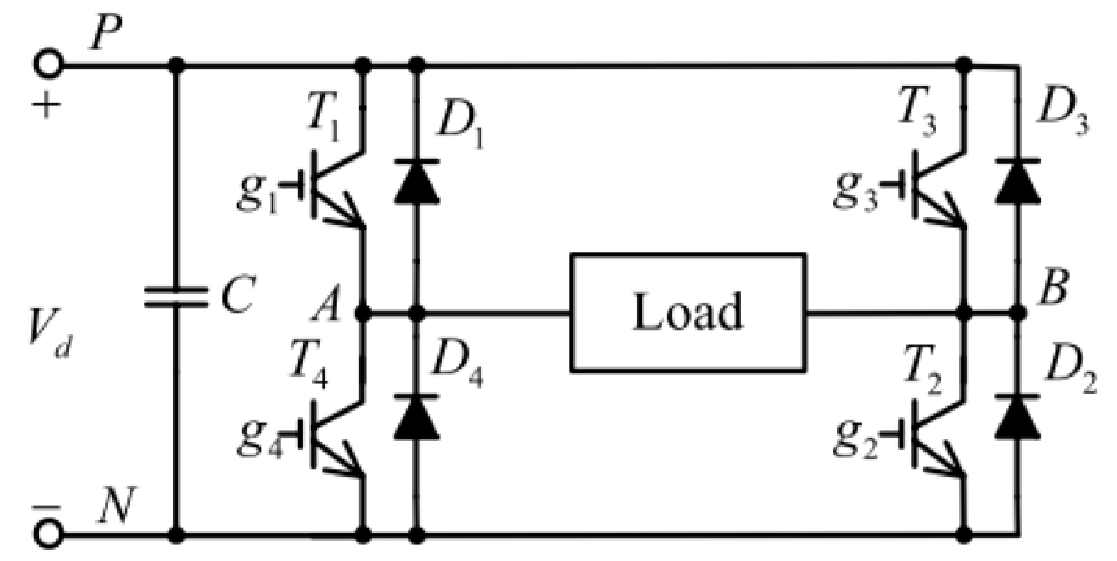
\includegraphics[width = 5in]{./Figures/h-bridge.pdf}
		\rule{35em}{3pt}
	\caption{Unit H Bridge}
	\label{fig:5}
\end{figure}

\section{Cascaded 9-level H Bridge}
The concept of series H-bridge inverter was first proposed by R. H. Baker and L. H. Banister in 1975.To overcome the drawbacks of Neutral-Point Clamped and Flying Capacitor topologies such as extra clamping diodes and capacitors, Marchesoni have proposed CHI.This modular structure has been subsequently extended for three-phase applications.\\
CHB-MLI is formed by the series connection of two or
more single-phase H-bridge inverters; hence the name H bridge is given . Each H-bridge corresponds to two
voltage source phase legs, where the line–line voltage is
the inverter output voltage. Therefore, three different
voltage levels i.e. +V,-V and 0 are generated using a single H-bridge
inverter.\\
 Series connection of N such bridges can produce 2N+1 levels in the output. This connection is termed as cascaded H-bridge multilevel inverter.
Each leg has only two possible switching states, to neglect
dc-link capacitor short-circuit. For two legs,four different switching states are possible, although two of them have redundant output voltage.\\
If E Volts voltage source is connected with a unit H bridge, it gives 3 levels (E,-E including 0 V) square wave, more precisely Quasi-square wave\ref{fig:3} with voltage peak of E volts.\\
\begin{figure}[htbp]
	\centering
		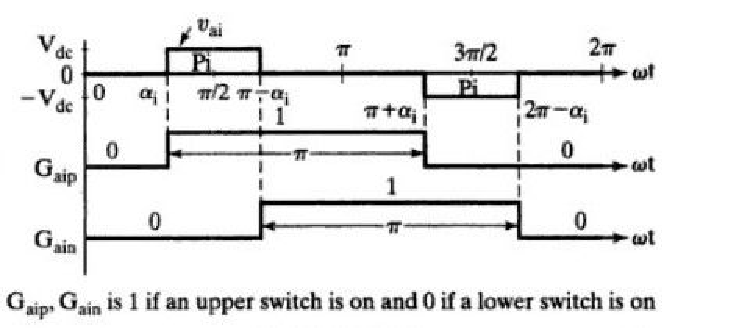
\includegraphics[width = 5in]{./Figures/quasi2.pdf}
		\rule{35em}{5pt}
	\caption{Quasi square wave}
	\label{fig:6}
\end{figure}\\

Considering above nomenclature in order to get 9-level staircase output two algorithms can be followed as described below.
\begin{description}
\item [Cascading 4 units of H bridge(equal source voltage) in series]
\item [Cascading 2 units of H bridge(unequal source voltage) in series]
\end{description}
\subsection{4 units of H bridge in series}
In this circuit \ref{fig8} 4 units of H bridge with equal value of source voltage are connected in series to get 9 levels of voltage as output such that when all the circuits give E outputs then we get total of 4E maximum and when all give -E volts as output we get -4E minimum collective. so we get a range of variable output from -4E to 4E.\\
However, this circuit is easy to apply but is large in size and has large no of switching resulting thus increase in temperature of the whole circuit. So, generally not reliable.\\
The ac outputs of each full-bridge inverter are connected in series such that the synthesized voltage waveform is the sum of the inverter outputs.
For an nine-level inverter which contains four separate sources, the per phase voltage is given by:
$$Van = Va1 + Va2 + Va3 + Va4 $$
The required circuit\ref{fig8} and expected waveforms \ref{fig:9} are as shown.\\
\begin{figure}[htbp]
	\centering
		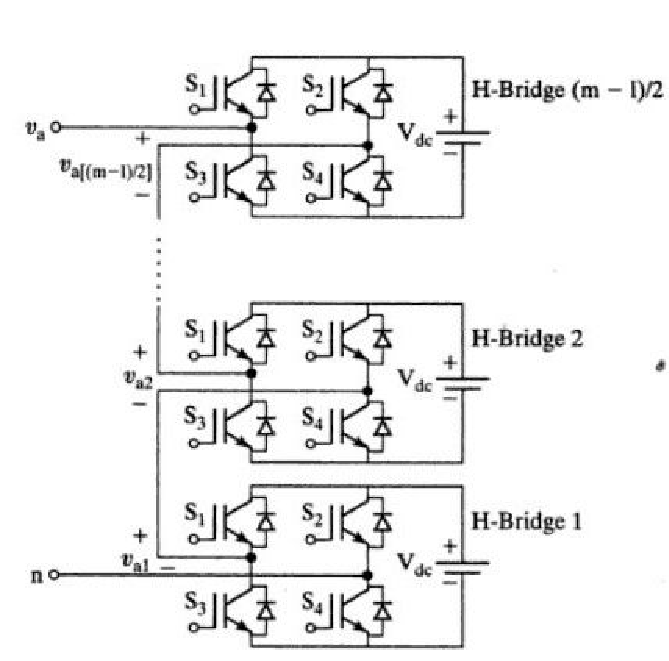
\includegraphics[width = 5in]{./Figures/ninecircuit.pdf}
		\rule{35em}{5pt}
	\caption{Cascaded Inverter Circuit(m=4)}
	\label{fig7}
\end{figure}
\begin{figure}[htbp]
	\centering
		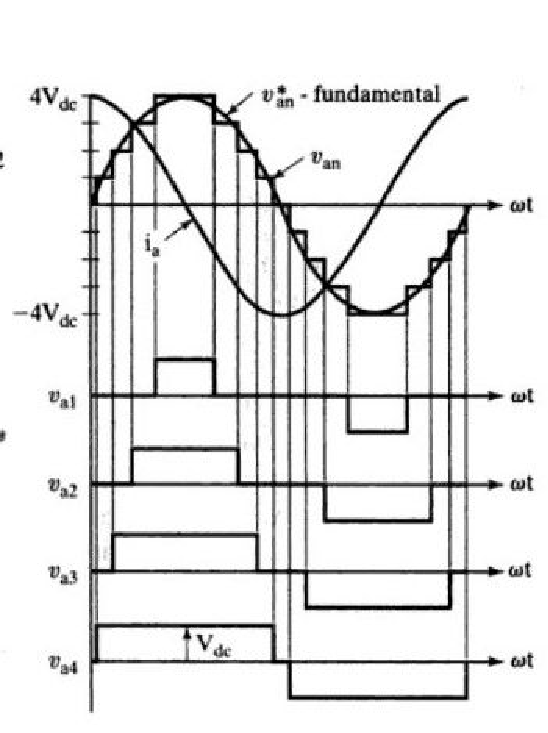
\includegraphics[width = 3in]{./Figures/ninewave.pdf}
		\rule{35em}{5pt}
	\caption{Cascaded Inverter nine levels of output voltage}
	\label{fig:8}
\end{figure}
By increasing the number of levels we can get a more sinusoidal waveform.
The conducting angles\ref{fig:9} $\theta1, \theta2, \theta3  and  \theta4$ can be chosen such that the voltage total harmonic distortion is minimum.
Generally, these angles are chosen so that predominant lower frequency harmonics 3, 5, 7, 11, and 13 are eliminated.\\
Thus, staircase waveform is obtained from the CHB multilevel
inverter which can be nearly sinusoidal as the number of levels has
increased, even without using filters. For a three-phase system, the
output voltage of three single-phase cascaded converters can be
connected in either $\star  or \delta$  configurations.

\subsection{2 units of H bridge in series}
In this circuit 2 units of H bridge one with source voltage of E and other with 3E are connected in series to get 9 levels of voltage as output.We get a range of variable output from -4E to 4E as shown:\\
 \begin{center}
	\begin{tabular}{ |p{4cm}||p{4cm}|p{4cm}|  }
		\hline
		\multicolumn{3}{|c|}{Table 9 levels of voltage} \\
		\hline
		3E source voltage contained H bridge&E source voltage contained H bridge&Value of voltage as resultant output\\
		\hline
		on & on & 4E\\
		on & off & 3E\\
		on & inverted & 2E\\
		off & on & E\\
		off & off & 0\\
		off & inverted & -E\\
		inverted & on & -2E\\
		inverted & off & -3E\\
		inverted & inverted & -4E\\
		\hline
	\end{tabular}
\end{center}
The output voltage of inverter is approximately sine wave with a Total Harmonic Distortion(THD) of less than 5 percent as each switch is working at 180 degree at its fundamental frequency.
\subsection{Features of Cascaded Inverter}
\begin{itemize}
\item The number of possible output voltage levels say m is more than twice the number of dc sources say s (m = 2s + 1).
\item Ability to reach higher output voltage and power levels.
\item Capable of reaching medium output voltage levels using lower rating switching components.
\item Repairing and replacement of faulty module is easy because of its high degree of modularity.
\item Selecting an appropriate control strategy in the case of fault conditions can bypass the fault module and can ensure continuous current to the load, bringing an almost continuous over all availability.
\item Ability to synthesize output voltage waveform with lesser value of total harmonic distortion.
\end{itemize}
\subsection{Limitations of Cascaded Inverter}
\begin{itemize}
\item Separate dc sources are required for each of the H-bridges.
\item As the number of levels increases, more number of switching devices are required in this configuration. This requirement further increases in three-phase configuration.
\end{itemize}
\section{Modulation Techniques for Multilevel Inverter}
 The inverter dc voltage input $V_d$ is usually fixed while its ac output voltage $V_(AB)$ can be adjusted by different modulation schemes.
Main objectives of modulation strategy are as follows:
\begin{itemize}
\item Capable of operating wide range of modulation index, preferably
from 0 to 1
\item Less switching loss with improved overall efficiency
\item Less THD in output voltage
\item Obtaining high magnitude of the output fundamental frequency
component
\item Easy for implementation for practical applications
\item Less computational burden and time
\end{itemize}
However, for the inverters used in high power applications,
THD, switching losses, switching capabilities and inverter
efficiency are the critical issues that must be taken into account in
performance evaluation.
\section{Classification of Modulation Techniques}
Based on switching frequency for computational work modulation techniques are classified as follows:
\begin{itemize}
\item Sinusoidal PWM and Space Vector PWM techniques for high switching frequency.
\item Selective Harmonic Elimination and Space Vector Control for fundamental switching frequency
\end{itemize}
\begin{figure}[htbp]
	\centering
		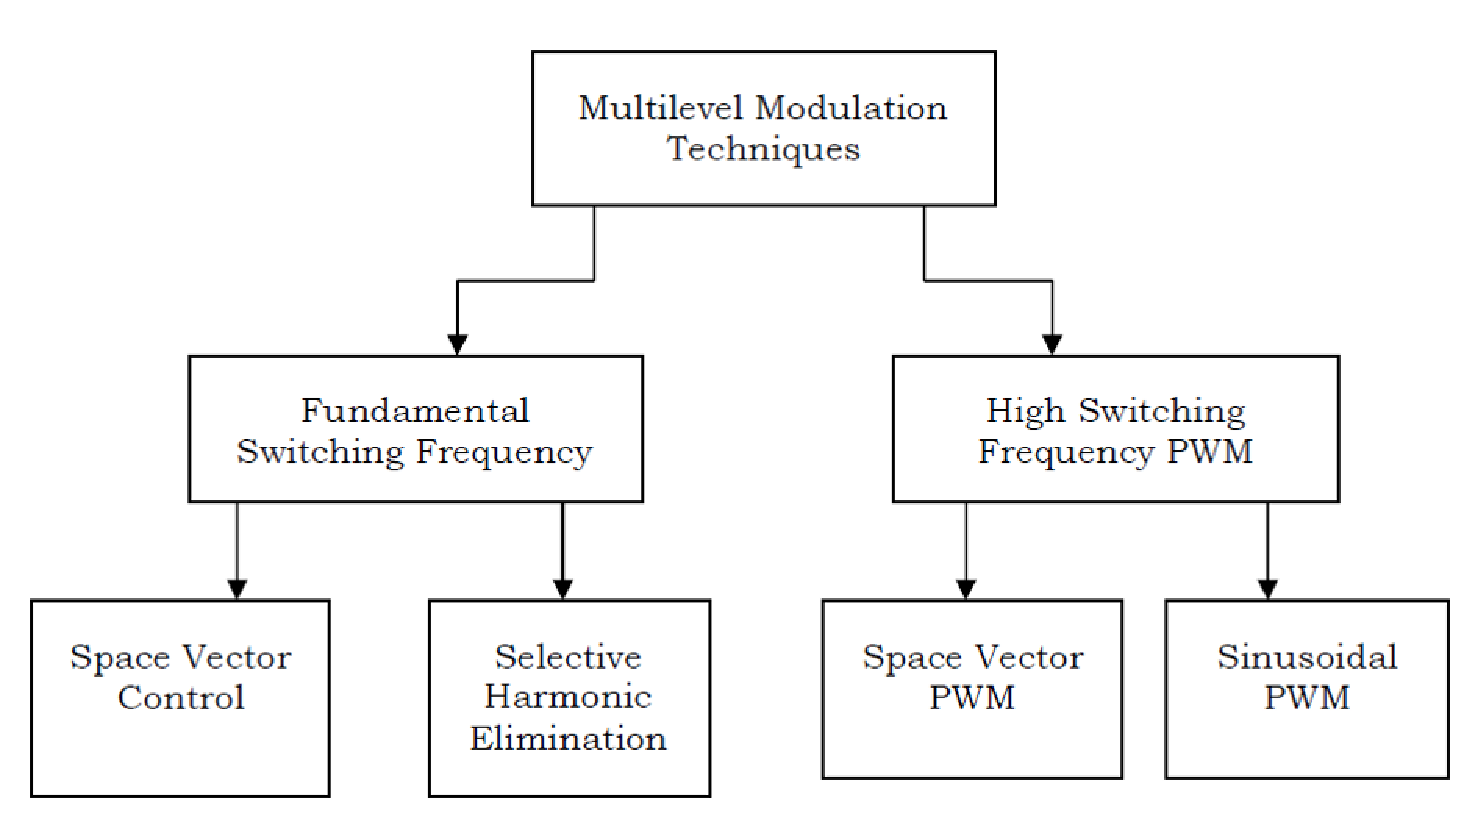
\includegraphics[width = 3.5in]{./Figures/Doc1.pdf}
		\rule{35em}{5pt}
	\caption{Classification of Modulation Techniques}
	\label{fig:9}
\end{figure}
\section{Sinusoidal PWM}
Carrier based sinusoidal PWM techniques which are employed in control CHBMLI can be
generally classified into two categories:
\begin{itemize}
\item Phase-shifted carrier based pulse width modulation technique.
\item Level-shifted carrier based pulse width modulation technique.
\end{itemize}
\subsection{Level-shifted carrier based PWM (LSCPWM) technique}
Level-shifted carrier based PWM (LSCPWM) technique is used to control neutral point clamped inverter and to control cascaded multilevel inverters. This technique has drawbacks such as uneven distribution of power among cells and high THD in output voltage and current wave forms.
LSCPWM is further divided into three categories:
\begin{itemize}
\item Phase Disposition (PD-PWM):
 wherein all the carrier signals are in same phase.
\item Phase Opposition Disposition (POD-PWM):
wherein the carrier signals above the zero are out of phase with those below the zero by $180^o$.
\item Alternative Phase Opposition Disposition (APOD-PWM):
 wherein the adjacent carrier signals are out of phase by $180^o$.
\end{itemize}
\subsection{Phase shifted carrier based PWM (PSCPWM) technique}
 Phase shifted carrier based pulse width modulation
(PSCPWM) technique is commonly used modulation technique for
control of cascaded multilevel inverters because of the following
reasons:
\begin{itemize}
\item Better harmonic profile of output voltage and current
wave-forms.
\item Even power distribution among levels.
\item Easy to implement independently. 
\end{itemize}
These advantages made PSCPWM technique popular compared to LSCPWM technique to control CHB multilevel inverters.\\
Generally, a multilevel inverter with m-level voltage requires $m-1$ triangular carriers. All the carriers have same frequency and same peak-to-peak amplitude with phase shift($\phi_(cr)$ )between adjacent carrier waves  and is given by
$$\phi_(cr)=\frac{360^o}{m-1} $$

The modulating signal is usually a three-phase sinusoidal wave
with adjustable amplitude and frequency. By comparing the
modulated wave $V_(mA)$ with the carrier waves gate signals are
generated.
 The fundamental voltage component in the inverter output
voltage can be controlled by modulation index $M_I$. Modulation index
is the ratio of maximum voltage value of modulating wave $V_m$ to
carrier wave voltage $V_(cr)$.
The modulation index $M_I$ is usually adjusted by varying $V_m$ by
keeping $V_(cr)$ fixed.
$$M_I=\frac{V_m}{V_(cr)}$$
Harmonics in the case the of high switching
frequency modulation techniques appears as side-bands around
carrier frequency produces high THD which results in trouble some
filtering.For the project case multi-carrier sinusoidal PWM technique is used.
